% Build on the outline below.  Cite by using \citep{Author2016} to add a
% parenthetical citation; use \citet{Author2016} to get a textual cite like
% this: Author (2016). 

\section{Plot Interaction Terms}

It has been well known for over a decade that models containing multiplicative interaction terms require particular care in interpretation \citep[see, e.g.,][]{Golder2003a, Braumoeller2004, Brambor2006, Kam2007a}.



\begin{figure}[htbp] 
  \caption{Logit Coefficients of Local Income Inequality by Respondent Income: Table 1, Model 1, From Replication Data}
  \label{F:coef.t1m1}
  \begin{center}
    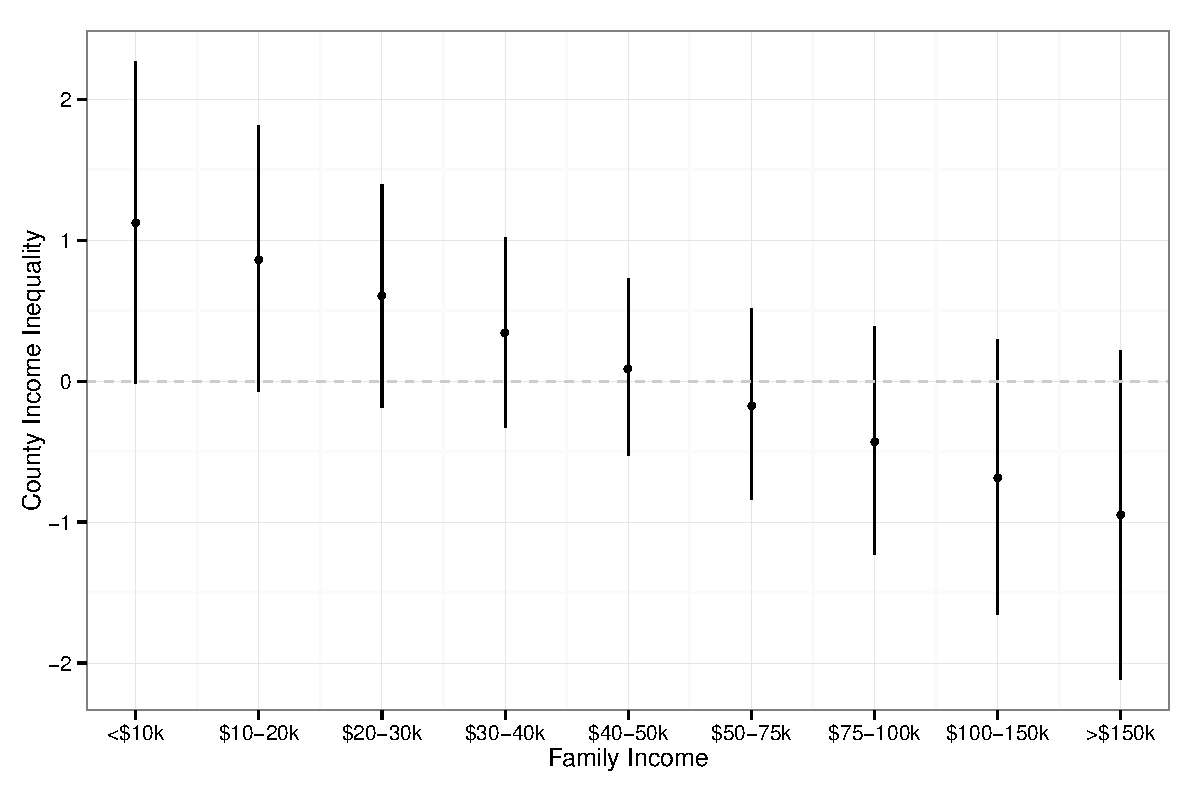
\includegraphics[width=5.25in]{../figures/07_plot_interaction_terms_t1m1.pdf}
  \end{center}
  \begin{footnotesize}
  \begin{tabular}{p{.1in} p{5.1in}}
  & \emph{Notes}: The coefficient for county income inequality fails to reach statistical significance for any observed level of respondent family income.
  \end{tabular}
  \end{footnotesize}
\end{figure}


% \begin{figure}[htbp] 
%   \caption{Logit Coefficients of Local Income Inequality by Respondent Income, Table B1, White Respondents, From Source Data with Missing Values Multiply Imputed}
%   \label{F:coef.b1m1}
%   \begin{center}
%     \includegraphics[width=5.25in]{../figures/07_plot_interaction_terms_b1m1_mi.pdf}
%   \end{center}
%   \begin{footnotesize}
%   \begin{tabular}{p{.1in} p{5.1in}}
%   & \emph{Notes}: The coefficient for county income inequality fails to reach statistical significance for any observed level of respondent family income.
%   \end{tabular}
%   \end{footnotesize}
% \end{figure}

